\documentclass[twocolumn,gsifonts,twoside]{gsipaper}
\usepackage{a4wide,gsiindex,helvet}
\usepackage[english]{babel}
\usepackage{amsmath,amsfonts,amssymb,verbatim,float}
\usepackage[]{graphicx} % Graphic files: pdf or jpg

% \usepackage{natbib}
\usepackage{hyperref}

\graphicspath{{./Images/}}




\begin{document}
%\author{Jacopo Lancione}
\title{\textbf{Deep Learning Project}} % TODO

\abstract{ % TODO
Qlo che ho fatto
Manifold hypothesis
how true is it relating
}

\shortauthor{Lancione, Jacopo}
\shorttitle{Deep Learning Final Project}

\author{Jacopo Lancione}            % first author
\address{Università di Torino, jacopo.lancione@edu.unito.it}

\maketitle




\section{Question and insights}
This work revolves around the latent representiation developed with autoencoders and how far the insight of the manifold hypothesis can be pushed with this respect. In other words, is there really a connection between the latent representation build by autoencoders and the supposed data manifold?

First, some comments on the intuition of the data manifold, because they will be the lighthouse of the following analysis. Intuition suggests that within the space of the features the actual meaningful data lies on an embedded manifold. So the data is expected to have some kind of structure. The easiest case to inspect this supposed structure is to use data that already suggests part of it and then verify if this is preserved in the representation developed by the autoencoder. For the sake of concreteness let us develop straight away the example at the basis of this work. The dataset used is MNIST  % TODO reference
, the feature space is the $28\times28$-dimensional space of all possible grey scale images. The data is hand-written digits and some structure of the data is suggested by the labels, i.e. the digits. Now the key argument: by moving on the supposed data manifold one would expect to reach all the instances of the same digit without crossing to another digit. Therefore different digits should be separated on the learned representation of such manifold, since starting from a data point labelled with digit 2 it would be awkward to be forced to go through a region of 7s to reach another instance of digit 2. This is the structure one would see preserved in a somewhat faithful representation of the data manifold.

The proposed argument infers that representations such as fig.~\ref{fig:vae} have little to do with the supposed data manifold, since in the encoding process they loose part of the structure of the data, which could result in an inefficient latent code.

\begin{figure}
  \centering
  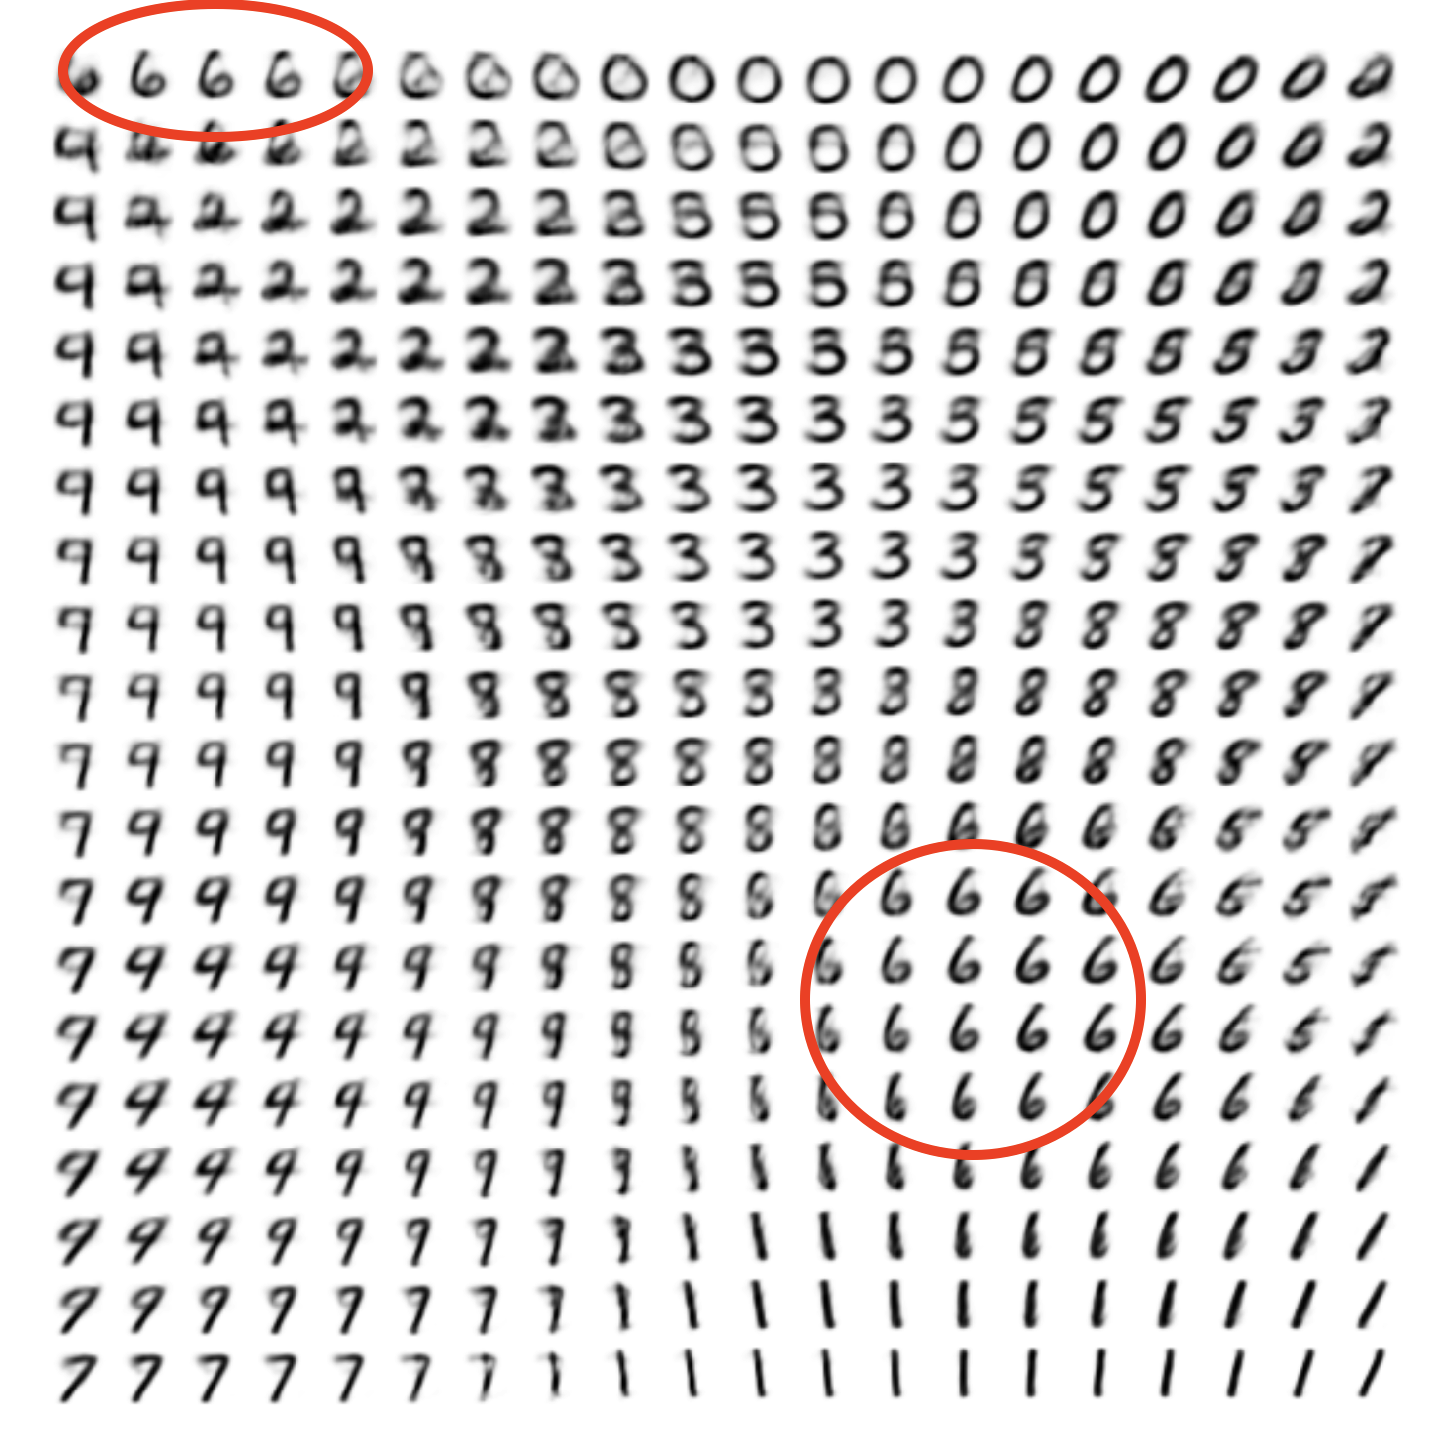
\includegraphics[width=.6\linewidth]{image_from_vae.png}
  \caption{\cite{Kingma2022}} % TODO
  \label{fig:vae}
\end{figure}


\section{Methods}
Qua descrivi solo i metodi utilizzati ma nn dire niente di $+$
(magari metti le foto delle immagini ricostruite dgli autoencoder)

autoencoder, denoising, pca
scrivi della tua implementazione e metti i dettagli dell'architettura magari in tabella

silhouette score
la cosa dei raggi di girazione


\section{Results}


\section{Conclusions}


\section{Future developments}
This work is intended as a qualitative analysis. There is an intrinsic lack of completeness in the exploration of the question posed. One such limitation in the methods regards the metrics used to choose the model for the analysis. Here the validation loss after training was chosen for this evaluation. However, it does not take into account the cases were the reconstructed image is more similar to the other class than the original label. This criterion is arguably more relevant than the validation loss itself, since the whole analysis revolves around the latent space organization of the data and a wrong \emph{recostruction of the label} (this is the metric proposed) is expected to imply a mispositioning in the latent representation.

Another critical aspect of the problem is the dimensionality of the latent space. The choice of taking it 2-dimensional is due to the argument that each figure has to live at least in a 2-dimensional space, since it has to take into account for rotations and stretches of the image. This is of course an approximation, since for a single label there is a higher variability that cannot be reduced to the aformentioned transformations. Therefore, a proper study across different latent space dimensions is certainly encouraged since one might expect the data manifold to be more approximated better in a higher dimensional latent space.

One further interesting discussion would relate the machine learning methods explored with more controlled algorithms of manifold identification. There exist many different non linear methods of manifold approximation that rely on geometrical arguments. An interesting one is named \emph{Manifold Sculpting} \cite{Gashler2007}
, whose objective is to transform the data while trying to preserve local relations such as distances and angles between neighbor points. This has been part of the original explorative analysis in this work of the different representations of the latent space, in the repository \url{https://github.com/jlancione/DeepLearningProject}
there is a single core implementation\footnote{Pseudocode in the paper \cite{Gashler2007} and reference implementation in the repository \url{https://github.com/Gabriele-Codega/Manifold_Sculpting}.
} in PyTorch of such algorithm but its computational complexity made it unfeasible to conduct a proper analysis with the available resources. 



%\bibliographystyle{plain}  
%\bibliography{Zotero} % Nn trova qlo di Gashler (ha 1 icona diversa...)

\begin{thebibliography}{99}
  \bibitem{Kingma2022}
  Kingma, D. P. \& Welling, M. Auto-Encoding Variational Bayes. Preprint at https://doi.org/10.48550/arXiv.1312.6114 (2022).

  \bibitem{Gashler2007}
  Gashler, M., Ventura, D. \& Martinez, T. Iterative Non-linear Dimensionality Reduction with Manifold Sculpting. in Advances in Neural Information Processing Systems vol. 20 (Curran Associates, Inc., 2007).

  \bibitem{Plaut2018}
  Plaut, E. From Principal Subspaces to Principal Components with Linear Autoencoders. Preprint at https://doi.org/10.48550/arXiv.1804.10253 (2018).
\end{thebibliography}












\end{document}
